\documentclass[a4paper, 12pt]{report}
\usepackage[T1]{fontenc} 
% \usepackage[icelandic]{babel}
\usepackage{latexsym,amssymb,amsmath,amsthm}
\usepackage{graphicx}
\usepackage[colorlinks=true,linkcolor=black,anchorcolor=black,citecolor=black,filecolor=black,menucolor=black,runcolor=black,urlcolor=black]{hyperref}
\usepackage{enumerate}
\usepackage{pgfplots}
\usepackage{nicefrac}
\usepackage{derivative}
\usepackage{setspace}
\usepackage{mathrsfs}
\usepackage{newtxtext, newtxmath}
\usepackage{tabularx}
\usepackage{authblk}

\usepackage{algorithm}
\usepackage{algpseudocodex}
\renewcommand\algorithmicprocedure{\textbf{procedure}}
\newcommand{\algorithmicendprocedure}{\algorithmicend\ \algorithmicprocedure}
\makeatletter
\newcommand\PROCEDURE[3][default]{%
  \ALC@it
  \algorithmicprocedure\ \textsc{#2}(#3)%
  \ALC@com{#1}%
  \begin{ALC@prc}%
}
\newcommand\ENDPROCEDURE{%
  \end{ALC@prc}%
  \ifthenelse{\boolean{ALC@noend}}{}{%
    \ALC@it\algorithmicendprocedure
  }%
}
\newenvironment{ALC@prc}{\begin{ALC@g}}{\end{ALC@g}}
\makeatother


\usepackage[hang,flushmargin]{footmisc}

\pgfplotsset{compat=1.17}
\setlength{\jot}{1em}

\title{\textsc{Simulating the Evolution of\\ Neural Pathways and Structures} \\ \vspace*{10mm} \Large Development Journal}
\author[1]{Kári Hlynsson}
\author[2]{Young Jun Lee}
\affil[1]{University of Iceland, Department of Mathematics}
\affil[2]{University of Oxford, Department of Biology}
\date{}

\newtheorem{theorem}{Theorem}
\newtheorem{corollary}{Corollary}
\newtheorem{proposition}{Proposition}

\theoremstyle{definition}
\newtheorem{definition}{Definition}
\newtheorem*{remark}{Remark}

\let\oldproofname=\proofname
\renewcommand{\proofname}{\rm\bf{\oldproofname}}


\begin{document}

\maketitle

\onehalfspacing
\newpage

\tableofcontents

\newpage
\chapter*{Index of notation}
\renewcommand{\arraystretch}{1.7}
\begin{table}[ht!]
    \centering
    \begin{tabularx}{\textwidth}{l X}
      \textsc{Abbreviation} & \textsc{Definition} \\
      $\mathscr E = [0;w] \times [0;h]$ & Environment with \emph{width} $w$ and \emph{height} $h$. The environment
                                           can also be expressed as the set of locations $\ell$ such that $\mathscr E = \{\ell := \langle x_i, y_j \rangle \mid x_i \in [0;w] \land y_j \in [0;h]\rangle\}$ \\
      $n$                                & Size of the population. \\
      $E = (e_x, e_y)$                  & An entity with $x$ and $y$ coordinates in the environment such that $\ell_{E} \in \mathscr E$ ($\ell_E$ is the location which corresponds to the entity's location) \\
      $\mathbf C = \{C_1, \ldots, C_k\}$ & The partition of $\mathscr E$ into $k$ chunks $C_1, \ldots, C_k$ such that $\bigcap_{i = 1}^k C_i = \emptyset$ and $\bigcup_{i = 1}^k C_i = \mathscr E$, i.e. the
                                            \emph{set of chunks} $\mathbf C$ forms a complete partition of $\mathscr E$. \\
      $\mathbf O = \{O_1, \ldots, O_n\}$ & The population, the set of all organisms present within the environment. \\
      $\theta_R = \frac{1}{\delta_R}$    & An organism's \emph{ray resolution}. The ray resolution is defined as the inverse of the angle between the uniformly spaced sensory rays, $\delta_R$ which construct 
                                           the organism's sensory field. The higher the value of $\theta_R$, the more rays in the sensory field and vice versa. \\
      $\mathcal P: \mathbf O \to \ell$   & Positional mapping. Returns vector representation of an entity's location at some point in time. Note that $\mathcal P$ is a random variable.
    \end{tabularx}
\end{table}

\newpage
\chapter*{Common Acronyms}
\begin{table}[ht!]
    \centering
    \begin{tabularx}{\textwidth}{l X}
      \textsc{Acronym} & \textsc{Definition} \\
      CBS & Chunk-Based System \\
      UGP & Undirected-Graph Partitioning \\
      BFS & Breadth-First Search
    \end{tabularx}
\end{table}


\newpage

\chapter{Theoretical basis}
\section{Note}
Hello there Jun

\noindent
This is an \textsc{\huge EXTREMELY} primitive draft.

\noindent
None of this final and subject to changes as we cooperate on this project.

\noindent
I also want to apologize for the common abbreviatons section, its a load of cowdung
but I feel we will need this to make our lives easier later on.

\chapter{Model outline}
\section{Model outline}
\subsection{Overview}
The aim of the model is to study the natural evolution of neural pathways in a population of organism
when exposed to survivalistic conditions. A rigid logical and syntactical foundation will make all succeeding
articulation on the model parameters and attributes easier. We therefore dedicate this first section towards
establishing a foundation of terms and definitions which we build on later.
\par The most critical aspects of the model we define here is the \emph{environment} and the \emph{entities} contained
therein. Neglecting any elevation, we define the environment as the bounded subset of the Cartesian plane, which we symbolize
$\mathscr E$ \footnote{Although elevation certainly plays a vital role in the foraging patterns of organisms in natural environments, we refrain
from its implementation as it only adds a level of complexity to the model design while having no immediate benefit for the simulation.}.
\par Contained within the environment are \emph{entities} which we can think of as actors within the simulation. The two types that occur
in this model are \emph{organisms} and \emph{food}. Again, a simple intuitive definition is that the organism is an individual of a species
present within the environment and nutrition is the foodstuffs which it consumes to gain energy and thus survive.
\par Entities can be divided into two types: \emph{organisms} and \emph{food}. What follows is simple: organisms are motile, can sense their surroundings
and consume food to gain energy. On the other hand, food has none of these qualities. We represent an entity as the object $E$, while organisms are denoted
$O$ and food by $F$.

\subsection{Sensory mapping of organisms}
One of the key characteristics of organisms is that they are able to sense their proximal surroundings and base their succeeding actions on the information they
have gathered on the environment. In this section we aim to establish a mathematical and syntactical foundation describing the sensory capabilities of organisms
which allows passing environmental data to the organism's neural network.
\par A convenient and well established method of sensory mapping is obtained through the use of \emph{raycasting} or \emph{raylines}, where several line segments
originating from the organism's point location are used as collision sensors which serve as sensors for distance. By calculating the distance of the intersection between
some rayline emitted by an organism and an entity in the field, a metric describing the \emph{sensory depth} from the organism to another entity is established.
\par To begin the formalization, we consider how to construct such a set of rays and what qualities it has.

\begin{definition}[Ray set]
    Let $\lambda \in \mathbb R^+$ and $t \in [0; 2\pi]$. Further suppose that an organism $O$ in an environment $\mathscr E$ with a present entity set $\mathbf E$ has the forward
    facing angle $\theta$. We define the \emph{ray set} of the organism as the linearly spaced vector $\mathbf R = \{r_1, \ldots, r_{\nu_{\mathbf R}}\}$ from $\left[\theta + \Delta_{\mathbf R}; \theta - \Delta_{\mathbf R}\right]$
    numbering $\nu_{\mathbf R}$ elements ($\nu_{\mathbf R}$ is called the \emph{ray number}). Furthermore, we define the quantity $\mathcal S_{\mathbf R} = 2 \Delta_{\mathbf R}$ as the \emph{span} of the ray set.
\end{definition}

\noindent
We now consider a function which returns the point locations of the rays along the sensory field from which we can construct line segments originating from the organism,
yielding the raylines.

\begin{definition}[Ray map function]
   The ray map function $\mathcal R_{\lambda}: \mathbf R \to \mathscr E$ is the bijective function from the set of rays $\mathbf R$ to the 
\end{definition}

\section{Simulation phases}
For your contemplation (Jun, if you're reading this): I've thought of dividing the simulation into a \emph{foraging phase}, where organisms roam around and collect food.
If they don't get any or deplete their energy, they die. Once the foraging phase is over, the \emph{reproductive phase} starts, where remaining energy is a measure of how
likely organisms are to find a partner and reproduce (this is of course a simplication, there are many other ways to go about this I'm sure). This way, we don't have to make
the reproduction itself an extreme pain (organisms having to find each other, etc.) This would mean that the reproductive phase is not carried out in the "plane" where the simulation
occurs but rather "off screen" where its just a bunch of calculations really.
\par On the other hand it might make for some really interesting data if we were to assign individuals genders and they would map their current energy level and the gender of individuals
in their sensory field and allow for them to reproduce "in the field" lol. Let me know what you think!

\section{Runtime optimization}
One of the run-ins we've had so far is determining how to design the sensory mapping capabilities of organisms within the environment. By sensory mapping, I am referring to the organism's ability to sense its
proximal surroundings, sensing the proximity and types of the various entities they may encounter. This will be fed into their neural network, which outputs some response which instructs the organism how to behave
given its current surroundings.
\par The first attempt I made was in the days where the environment was grid-based instead of a float-based environment. There, sensory mapping was quite easy as all that had to be done was inspect the proximal tiles
and check for the entity type present in the tile. This is not possible in the float-based environment, so we propose another solution.
\par An excellent idea you came up with was the idea of partitioning the environment into separate chunks, which organisms restrict their sensory mapping to unless there sensory fields intersect another adjacent chunk
(more on that later). We will start by discussing this idea, which as you will see, will be of great use.

\subsection{Chunk system}
In this section, we will be doing a mathematical analysis of the chunk system to see how it will benefit the simulation. To start off, we inspect what fundamental laws apply to this system.

\begin{proposition}
    Let $\mathscr E$ be an environment paritioned into $k$ chunks such that $\mathbf C = \{C_1, \ldots, C_k\}$. The probability of an entity being present in a generic chunk $C_i$ equals $1/k$, i.e.
    \[
        \textnormal{Pr}\{E \in C_i\} = \frac 1k
    \]
\end{proposition}

\begin{proof}
    Let $\mathscr E$ be the space $[0; w] \times [0;h]$ with $\text{area}(\mathscr E) = wh$ and the partition $\mathbf C$. Under the assumption that the chunks
    are of uniform size, we assume
    \[
        \text{area}(C_i) = \frac{\text{area}(\mathscr E)}{k} \tag{\textasteriskcentered}
    \]
    for all $C_i \in \mathbf C$ where $i \in [1; k]$. Under conventional probability theory, we can express the probability of an entity being in a generic chunk as
    the area of that particular chunk over the area of the environment, i.e.
    \begin{align*}
        \text{Pr}\{E \in C_i\} &= \frac{|C_i|}{|\mathscr E|} \\
                               &= \frac{\text{area}(C_i)}{\text{area}(\mathscr E)} \\
                               &= \frac{1}{k}
    \end{align*}
    The result of the calculations above are immediate of the definition of the area of the chunks, which is derived in (\textasteriskcentered).
\end{proof}

\begin{definition}[Chunk load]
    The random variable $\mathcal L$, or the \emph{chunk load} of some generic chunk $C_i$,
    denotes the number of entities contained within the chunk. Immediate of proposition 1,
    we have that $\mathcal L \sim \text{Bin}(n, 1/k)$, where $n$ is the total number of entities
    in the environment. \footnote{Note that this assumes the uniform distribution of entities within
    the environment, which is obviously true. This is because there is no logical restraint on where an
    entity can be at any given time, i.e. there is not a consistent probabilistic hindrance in an entity having a certain position.}
\end{definition}

\begin{figure}[ht!]
    \centering
    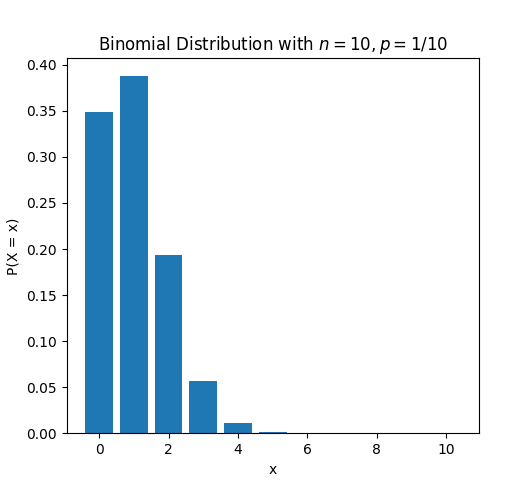
\includegraphics[width=0.6\textwidth]{img/binomialdistribution.png}
    \caption{An example binomial distribution}
\end{figure}

\noindent It should come as no surprise that the ratio of chunks to the population size has some impact on the max chunk load,
as can be seen in the picture below.

\begin{figure}[ht!]
    \centering
    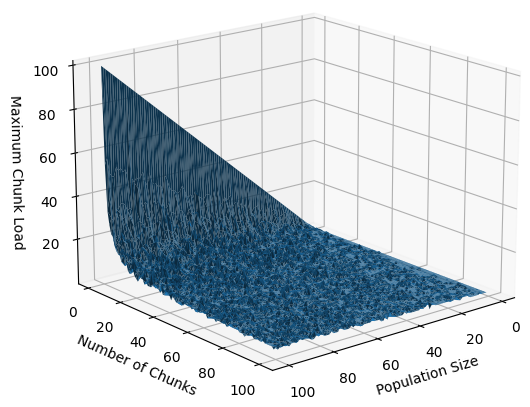
\includegraphics[width=0.6\textwidth]{img/mcl_simulation.png}
    \caption{$\mathcal L_{\max}$ by population size and number of chunks}
\end{figure}

\section{Adjacent chunk loading and critical boundary}
We define the \emph{critical boundary} of a chunk $C_i$ as the area in which the sensory field of a organism with a range of possible
positions intersects an adjacent chunk.


\section{Performance comparison}
In this section we compare the CBS versus non-CBS runtime performance to obtain a metric description
of performance improvements as a result of the CBS implementation.
\begin{algorithm}[ht!]
    \caption{Comparisonal simulation of CBS versus non-CBS runtime}
    \begin{algorithmic}[1]
        \Require The chunk set $\mathbf C$ which partitions $\mathscr E$ into $k$ disjoint
        subsets $C_1, \ldots, C_k$ where $|\mathbf C| = k$. Entity set $\mathbf E$ within $\mathscr E$
        where $|\mathbf E| = N$ with organism subset $\mathbf O$ such that $|\mathbf O| = n$.
        \Procedure{CbsComparison}{$\mathbf C$, $\mathbf E$}
        \State cost$_{\text{CBS}} \leftarrow 0$ \Comment{Amortized CBS cost}
        \State cost$_{\text{non-CBS}} \leftarrow n(N - 1)$ \Comment{Amortized non-CBS cost}
        \For{$C_i \in \mathbf C$}
            \State Assign $C_i$ chunk load $\mathcal L_{C_i} \sim \text{Bin}(N, 1/k)$ by random process
            \State $n_{O \in C_i} = |\{O \in \mathbf O \mid O \in C_i\}|$ \Comment{$n_{O \in C_i} \leq n$}
            \State cost$_{\text{CBS}} \leftarrow$ cost$_{\text{CBS}} \mathrel{+}= n_{O \in C_i} (\mathcal L_{C_i} - 1)$
        \EndFor
        \State cost$_{\text{CBS}} \leftarrow$ cost$_{\text{CBS}} \mathrel{+}= k$
        \EndProcedure
    \end{algorithmic}
\end{algorithm}
\par
\noindent \textsc{Note:} This algorithm does not take ACL into account, which we need to implement.

\appendix

\newpage

\chapter{Preliminaries}
\begin{definition}[Probability]
    Let $\omega$ be some event from the probability space $\Omega$. We represent
    the probability of the event $\omega$ occuring using the notation $\text{Pr}\{\omega\} = x$
    where $x \in [0;1]$.
\end{definition}

\begin{definition}[Random variable]
    A random variable $X$ is the mapping from the probability space $\Omega$ to the real number
    line, i.e. $X: \Omega \to \mathbb R$.
\end{definition}

\begin{remark}
    An example of a random variable is the varying height of a population, where $\Omega$ is the
    space of all possible outcomes and the random variable $H$ (height) is for example 180 cm, or 157 cm. 
\end{remark}

\begin{definition}[Expected value]
    Let $X$ be a random variable. The expected value is denoted $\mathbb E[X]$.
\end{definition}

\begin{definition}[Probability distribution]
    Let $X$ be a random variable. When it follows for example the Poisson distribution, we write
    $X \sim \text{Poisson}(\lambda)$.
\end{definition}

\end{document}